\documentclass[UTF8]{ctexart}
\usepackage{geometry}
\geometry{a4paper, margin=2.5cm}
\usepackage{graphicx}
\usepackage{listings}
\usepackage{xcolor}
\usepackage{float}
\usepackage{hyperref}
\usepackage{amsmath}
\usepackage{amssymb}
\usepackage{bm}
\usepackage{caption}
\hypersetup{colorlinks=true, linkcolor=blue, urlcolor=blue}
\graphicspath{{D:/code/LATEX/Conmmunication}}

\lstset{
    basicstyle=\ttfamily\small,
    breaklines=true,
    frame=single,
    numbers=left,
    numberstyle=\tiny,
    tabsize=4,
    language=MATLAB,
    keywordstyle=\color{blue},
    commentstyle=\color{green!60!black},
    stringstyle=\color{red}
}

\title{\textbf{数字调制实验}}
\author{}

\begin{document}
\maketitle

\begin{center}
    \textbf{班级：}2024217802\quad \textbf{姓名：} 严子竣\quad \textbf{学号：}2024212622
\end{center}

\section{实验目的}
\begin{enumerate}
    \item 掌握 M-QAM 调制解调的基本原理，理解星座图映射与格雷编码。
    \item 基于复包络和正交信号空间，在 AWGN 信道下仿真 16-QAM 系统的收发过程。
    \item 统计并绘制误比特率（BER）、误符号率（SER）和误帧率（BLER）随 \(E_b/N_0\) 变化的曲线。
    \item 推导 16-QAM 在 AWGN 信道下的理论 BER 精确表达式，与仿真结果进行对比验证。
    \item 理解 BLER 与 SER 之间的理论关系。
\end{enumerate}

\section{实验原理}

\subsection{M-QAM 调制与解调}
M-QAM（正交幅度调制）是一种同时利用幅度和相位携带信息的数字调制方式。对于 \(M=16\) 的矩形 QAM，每个符号携带 \(k = \log_2 M = 4\) 个比特。将每 4 个比特分为两组，每组 2 个比特，分别映射到同相（I）和正交（Q）支路的 4 个电平上，形成复包络信号。

发送符号可表示为：
\begin{equation}
    x = (x_I + j \cdot x_Q) \cdot K
\end{equation}
其中 \(x_I, x_Q \in \{\pm 1, \pm 3\}\)，\(K = 1/\sqrt{10}\) 为平均能量归一化因子。实验采用格雷编码（Gray Coding）进行比特-符号映射，以最小化相邻符号间的误比特数。

\subsection{AWGN 信道模型}
接收信号为发送符号叠加加性白高斯噪声：
\begin{equation}
    y = x + n
\end{equation}
其中 \(n \sim \mathcal{CN}(0, N_0)\) 为复高斯噪声，\(N_0\) 为噪声功率谱密度。信噪比定义为：
\begin{equation}
    \frac{E_b}{N_0} \text{ (dB)} = 10\log_{10}\left(\frac{E_s/k}{N_0}\right)
\end{equation}
其中 \(E_s = 1\) 为归一化符号能量。

解调采用最大似然（ML）准则，即在星座图中寻找与接收符号欧氏距离最近的星座点作为判决输出。

\subsection{理论误码率精确计算}
对于 16-QAM 矩形星座图（Gray 编码），每符号的 4 个比特中，前两个比特（I 路）和后两个比特（Q 路）具有相同的错误概率结构。在 AWGN 信道下，单个比特的错误概率精确表达式如下。

定义 \(d_{\min} = 2/\sqrt{10}\) 为星座点之间的最小欧氏距离，噪声方差 \(\sigma^2 = N_0/2\)。令：
\begin{equation}
    x = \sqrt{\frac{d_{\min}^2}{2N_0}}
\end{equation}
则 I 路（或 Q 路）的两个比特各自的误比特率分别为：

\begin{equation}
    P_{b1} = \frac{1}{2}\left[ Q\left(\sqrt{\frac{9d_{\min}^2}{2N_0}}\right) + Q\left(\sqrt{\frac{d_{\min}^2}{2N_0}}\right) \right]
    \label{eq:Pb1}
\end{equation}
\begin{equation}
    P_{b2} = Q\left(\sqrt{\frac{d_{\min}^2}{2N_0}}\right) + \frac{1}{2}\left[ Q\left(\sqrt{\frac{9d_{\min}^2}{2N_0}}\right) - Q\left(\sqrt{\frac{25d_{\min}^2}{2N_0}}\right) \right]
    \label{eq:Pb2}
\end{equation}
其中 \(Q(\cdot)\) 为高斯 Q 函数。16-QAM 的总平均理论误比特率为：
\begin{equation}
    P_b = \frac{P_{b1} + P_{b2}}{2}
    \label{eq:BER_theory}
\end{equation}

\subsection{理论误符号率与误帧率}
理论误符号率的表达式为：
\begin{align}
    P_s &=1-(1-P_{4ASK})^2\\
    &= 1 - \left(1 - \frac{3}{2} Q\left(\sqrt{\frac{E_s}{5N_0}}\right)\right)^2
    \label{eq:SER_theory}
\end{align}

若每帧包含 \(N\) 个符号，且各符号错误相互独立，则误帧率（BLER）与误符号率的关系为：
\begin{equation}
    \text{BLER} = 1 - (1 - P_s)^N\approx NP_s
    \label{eq:BLER_theory}
\end{equation}

\section{仿真参数设置}

本次实验的仿真参数如下：
\begin{table}[H]
    \centering
    \caption{仿真参数配置}
    \begin{tabular}{|c|c|}
        \hline
        \textbf{参数} & \textbf{数值} \\
        \hline
        调制阶数 \(M\) & 16 \\
        \hline
        每符号比特数 \(k\) & 4 \\
        \hline
        每帧符号数 \(N_{\text{sym}}\) & 1000 \\
        \hline
        每帧比特数 & 4000 \\
        \hline
        每信噪比帧数 \(N_{\text{frames}}\) & 100 \\
        \hline
        信噪比范围 \(E_b/N_0\) (dB) & 0, 2, 4, 6, 8, 10, 12, 14 \\
        \hline
        星座图归一化因子 & \(1/\sqrt{10}\) \\
        \hline
    \end{tabular}
\end{table}

\section{仿真结果与分析}

\subsection{误码性能曲线}
通过蒙特卡洛仿真，统计了不同 \(E_b/N_0\) 下的 BER、SER 和 BLER，并与理论曲线进行对比。仿真结果如图 \ref{fig:MQAM} 所示。

\begin{figure}[H]
    \centering
    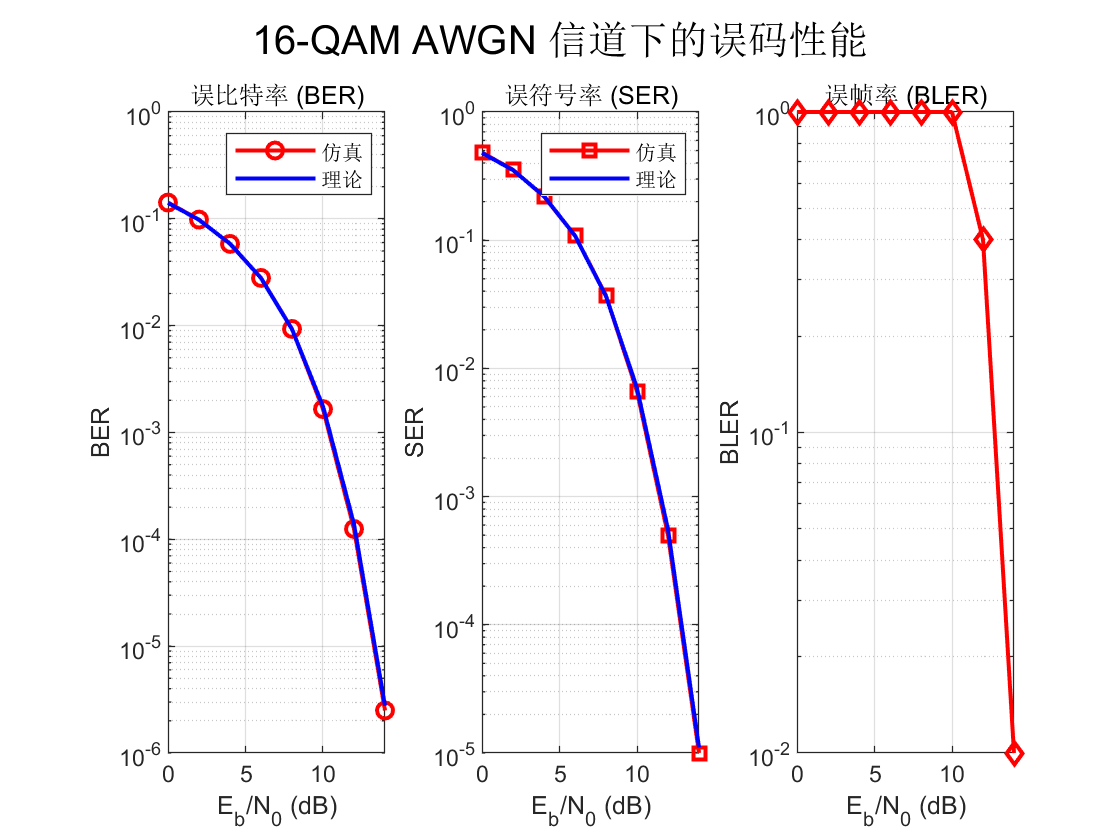
\includegraphics[width=\textwidth]{MQAM.png}
    \caption{16-QAM 在 AWGN 信道下的误码性能（BER、SER、BLER）}
    \label{fig:MQAM}
\end{figure}

\subsection{结果讨论}

\textbf{1. 误比特率（BER）分析}

图 \ref{fig:MQAM} 左图展示了 BER 随 \(E_b/N_0\) 的变化曲线。可以观察到仿真结果与理论精确值高度吻合，验证了实验代码中调制、解调、噪声生成及统计过程的正确性。在低信噪比区域（\(E_b/N_0 < 4\) dB），BER 较高（\(\sim 10^{-1}\)），随着信噪比增加，BER 呈瀑布状下降。在 \(E_b/N_0 = 14\) dB 时，BER 降至 \(\sim 10^{-5}\) 量级。

\textbf{2. 误符号率（SER）分析}

图 \ref{fig:MQAM} 中图展示了 SER 的变化趋势。由于理论 SER 表达式为近似公式，在高信噪比下与仿真值高度一致，低信噪比下略有偏差，但整体趋势吻合良好。SER 始终高于 BER，符合“每符号包含 4 个比特，符号错误概率大于单个比特错误概率”的预期。

\textbf{3. 误帧率（BLER）分析}

图 \ref{fig:MQAM} 右图展示了 BLER 的仿真结果。由于每帧包含 \(N_{\text{sym}} = 1000\) 个符号，只要帧内任一符号出错即导致整帧错误，因此 BLER 显著高于 SER。在 \(E_b/N_0 = 14\) dB 时，SER 已降至 \(10^{-5}\) 量级，但由于帧长较大，BLER 仍处于 \(\sim 10^{-2}\) 量级。这一结果与式 \eqref{eq:BLER_theory} 的理论预期一致。

\section{实验总结}

本次实验完成了 16-QAM 在 AWGN 信道下的完整链路仿真，涵盖比特生成、星座图映射（Gray 编码）、复包络调制、AWGN 信道加噪、ML 硬判决解调以及误码统计。

实验结果包括：
\begin{enumerate}
    \item 实现了基于复包络和正交信号空间的正交幅度调制仿真框架。
    \item 精确计算了 16-QAM 的理论误比特率，采用了公式 \eqref{eq:Pb1} 和 \eqref{eq:Pb2} 给出的精确 Q 函数表达式，仿真值与理论值高度一致，验证了精确理论的正确性。
    \item 完整统计并绘制了 BER、SER 和 BLER 三条性能曲线。
\end{enumerate}

\end{document}